\documentclass[tikz,border=10pt]{standalone}
\usetikzlibrary{shapes.geometric, arrows.meta, positioning, calc,
                shapes.multipart, backgrounds, shadows}

\begin{document}
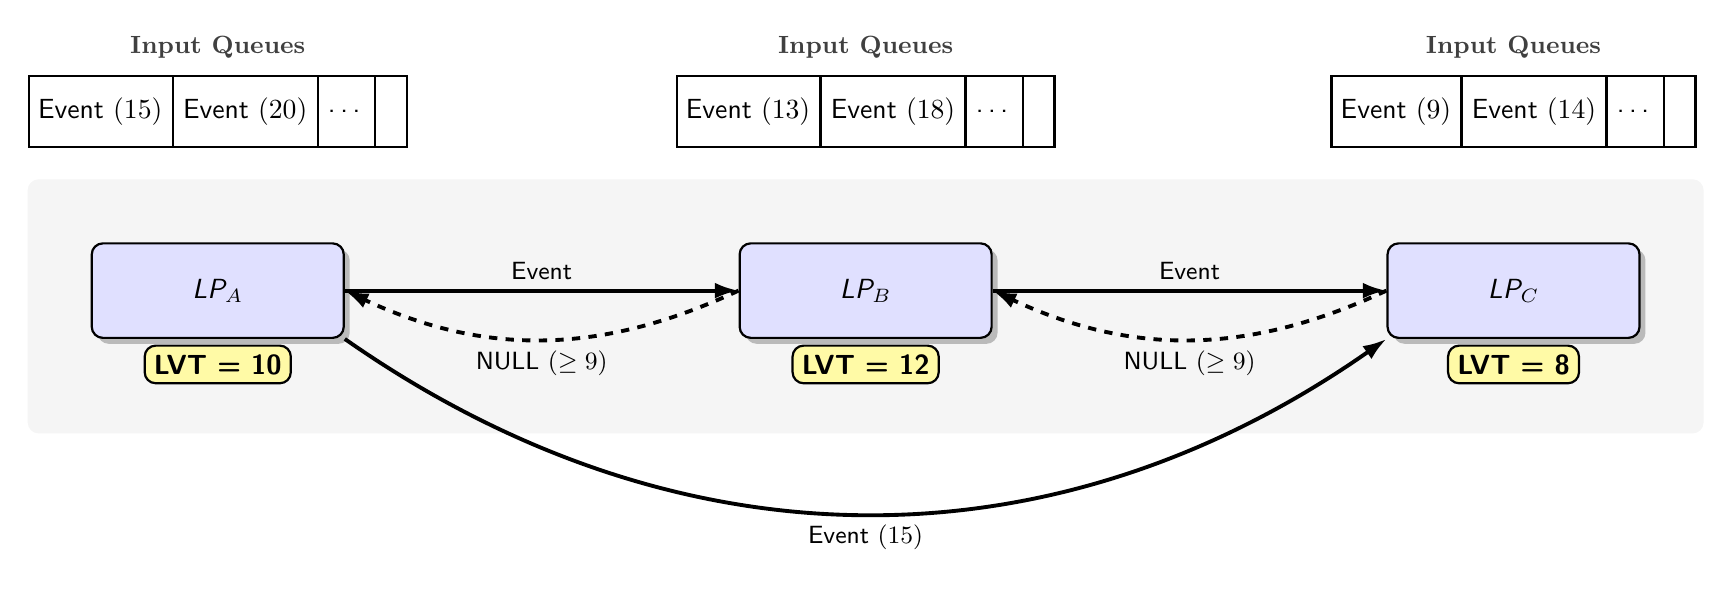
\begin{tikzpicture}[
    font=\sffamily,
    thick,
    component/.style={
        draw=black,
        fill=blue!12,
        rounded corners,
        minimum width=3.2cm,
        minimum height=1.2cm,
        align=center,
        drop shadow
    },
    lvtbox/.style={
        draw=black,
        fill=yellow!35,
        rounded corners,
        minimum width=2.2cm,
        align=center,
        below=2pt of #1
    },
    queue/.style={
        draw=black,
        fill=none,
        rectangle split,
        rectangle split parts=4,
        rectangle split horizontal=true,
        minimum height=0.9cm,
        align=center
    },
    msg/.style={
        -{Latex[length=3mm,width=2mm]},
        line width=1.4pt
    },
    nullmsg/.style={
        msg,
        dashed
    },
    label/.style={
        font=\bfseries\small,
        color=gray!50!black
    }
]

% --- LP NODES -------------------------------------------------

\node[component] (A) at (0,0) {$\emph{LP}_A$};
\node[component, right=5cm of A] (B) {$\emph{LP}_B$};
\node[component, right=5cm of B] (C) {$\emph{LP}_C$};

% --- LVT BOXES ------------------------------------------------

\node[draw, fill=yellow!35, rounded corners, below=2pt of A] (lvtA) {$\textbf{LVT = 10}$};
\node[draw, fill=yellow!35, rounded corners, below=2pt of B] (lvtB) {$\textbf{LVT = 12}$};
\node[draw, fill=yellow!35, rounded corners, below=2pt of C] (lvtC) {$\textbf{LVT = 8}$};

% --- INPUT QUEUES ---------------------------------------------

\node[queue, above=1.2cm of A] (QA) {
    \nodepart{one} Event $(15)$
    \nodepart{two} Event $(20)$
    \nodepart{three} \dots
    \nodepart{four}
};
\node[label, above=2pt of QA] {Input Queues};

\node[queue, above=1.2cm of B] (QB) {
    \nodepart{one} Event $(13)$
    \nodepart{two} Event $(18)$
    \nodepart{three} \dots
    \nodepart{four}
};
\node[label, above=2pt of QB] {Input Queues};

\node[queue, above=1.2cm of C] (QC) {
    \nodepart{one} Event $(9)$
    \nodepart{two} Event $(14)$
    \nodepart{three} \dots
    \nodepart{four}
};
\node[label, above=2pt of QC] {Input Queues};

% --- NORMAL EVENT FLOW ----------------------------------------

\draw[msg] (A.east) -- node[midway, above] {\small Event} (B.west);
\draw[msg] (B.east) -- node[midway, above] {\small Event} (C.west);

% --- NULL MESSAGE EXCHANGES (LOOKAHEAD INFORMATION) ------------

\draw[nullmsg, bend left=25]
    (B.west) to node[midway, below] {\small NULL $(\geq 9)$} (A.east);

\draw[nullmsg, bend left=25]
    (C.west) to node[midway, below] {\small NULL $(\geq 9)$} (B.east);

% --- SAFE EVENT PROPAGATION EXAMPLE ----------------------------

\draw[msg, bend right=35]
    (A.south east) to node[midway, below] {\small Event $(15)$} (C.south west);

% --- VISUAL GROUPING BACKGROUND --------------------------------

\begin{scope}[on background layer]
    \fill[gray!8, rounded corners]
        ($(A.north west)+(-0.8,0.8)$)
        rectangle
        ($(C.south east)+(0.8,-1.2)$);
\end{scope}

\end{tikzpicture}
\end{document}

